\documentclass{article}
\usepackage[margin=1in]{geometry}
\usepackage{amsmath,amsthm,amssymb}
\usepackage{bbm,enumerate,mathtools}
\usepackage{tikz,pgfplots}
\usepackage{chessboard}
\usepackage[hidelinks]{hyperref}
\usepackage{multicol} % Problem 35
\usepackage{xstring} % Difficulty command
\usetikzlibrary{shapes.geometric}

\newenvironment{question}{\begin{trivlist}\item[\textbf{Question.}]}{\end{trivlist}}
\newenvironment{note}{\begin{trivlist}\item[\textbf{Note.}]}{\end{trivlist}}
\newenvironment{references}{\begin{trivlist}\item[\textbf{References.}]}{\end{trivlist}}
\newenvironment{related}{\begin{trivlist}\item[\textbf{Related.}]\end{trivlist}\begin{enumerate}}{\end{enumerate}}

\newcommand\score[1]{
\pgfmathsetmacro\pgfxa{#1+1}
\tikzstyle{scorestars}=[
  star,
  star points=5,
  star point ratio=2.25,
  draw,
  inner sep=3pt,
  anchor=outer point 5
]
  \begin{tikzpicture}[baseline]
    \draw[opacity=0] (0,-0.5) rectangle (0,0.2); % Workaround for whitespace at the bottom.
    \foreach \i in {1,...,4} {
      \pgfmathparse{(\i<=#1?"yellow":"gray")}
      \edef\starcolor{\pgfmathresult}
      \draw (\i*4.5ex,0) node[name=star\i,scorestars,fill=\starcolor]  {};
    }
  \end{tikzpicture}
}

\newcommand{\difficulty}[1]{%
  \IfEqCase{#1}{%
      {1}{
        
\begin{tikzpicture}[scale=0.7, baseline=0.9mm]%
          \definecolor{slopegreen}{rgb}{0.0, 0.5, 0.0}%
          \fill[slopegreen] (0.5,0.5) circle (0.5);%
        \end{tikzpicture}%
      }%
      {2}{
        
\begin{tikzpicture}[scale=0.7, baseline=0.9mm]%
          \definecolor{slopeblue}{rgb}{0.0, 0.44, 1.00}
          \fill[slopeblue] (0,0) rectangle (1,1);%
        \end{tikzpicture}%
      }%
      {3}{
\begin{tikzpicture}[scale=0.7, baseline=0.9mm]\fill (0,0.5)--(0.5, 0)--(1,0.5)--(0.5,1)--cycle; \end{tikzpicture}}%
      {4}{
\begin{tikzpicture}[scale=0.7, baseline=0.9mm]\fill (0.25,0)--(0,0.5)--(0.25,1)--(0.5,0.5)--cycle; \fill (0.75,0)--(0.5,0.5)--(0.75,1)--(1,0.5)--cycle;\end{tikzpicture}}%
      % you can add more cases here as desired
  }[\PackageError{difficulty}{Undefined difficulty level: #1}{}]%
}%
\newcommand{\rating}[2]{\difficulty{#1}\\\score{#2}\\}


\begin{document}

\rating{2}{2}
Consider a frog hopping on a circular collection of $n$ lily pads. The frog hops to
any lily pad, and then hops with increasing steps. At the $k$-th step, the frog
looks $k$ steps in the clockwise direction and $k$ steps in the counterclockwise
direction and hops to whatever lily pad she has visited less. If there is a tie,
she hops in the clockwise direction.

\begin{figure}[ht!]
  \centering
  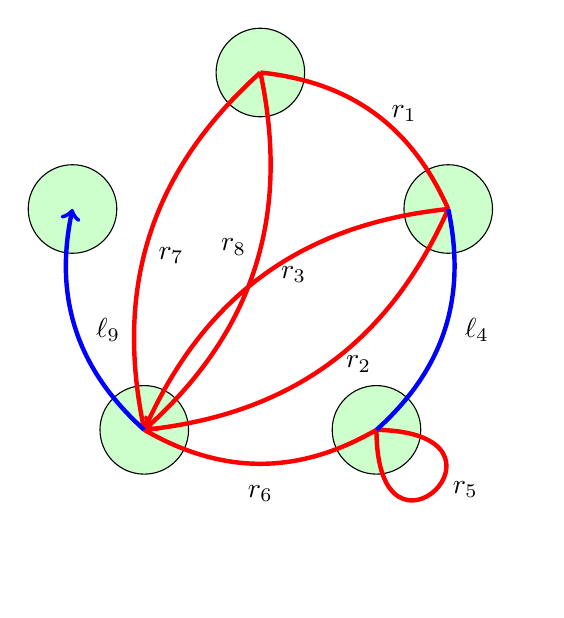
\begin{tikzpicture}
    % create the node
    \node[minimum size=5cm,regular polygon,regular polygon sides=5] (a) {};

    % draw a black dot in each vertex
    \foreach \x in {1,2,...,5} \draw[fill=green!20] (a.corner \x) circle[radius=16pt];
    \draw[red, ultra thick, ->]
      (a.corner 1) to[bend left] node[circle, black, right] {$r_1$} (a.corner 5)
      (a.corner 5) to[bend left] node[circle, black, right] {$r_2$} (a.corner 3)
      (a.corner 3) to[bend left] node[circle, black, right] {$r_3$} (a.corner 5)
      (a.corner 4) to[in=270, out=359, min distance=20mm] node[circle, black, right] {$r_5$} (a.corner 4)
      (a.corner 4) to[bend left] node[circle, black, below] {$r_6$} (a.corner 3)
      (a.corner 3) to[bend left] node[circle, black, below right] {$r_7$} (a.corner 1)
      (a.corner 1) to[bend left] node[circle, black, above left] {$r_8$} (a.corner 3)
    ;
    \draw[blue, ultra thick, ->]
      (a.corner 5) to[bend left] node[circle, black, right] {$\ell_4$} (a.corner 4)
      (a.corner 3) to[bend left] node[circle, black, right] {$\ell_9$} (a.corner 2)
    ;
  \end{tikzpicture}
  \caption{For $n = 5$, all lily pads will have been reached after nine hops.}
\end{figure}

\begin{question}
  How many hops does it take to reach all lily pads?
\end{question}

\begin{related}
  \item What if ties are broken by hopping in the same direction instead of
  hopping clockwise?
  \item What if instead of hopping with steps $1, 2, 3, \dots$, a different
  sequence is used?
  \item How many positions are reached exactly once?
  \item If the hops are in a random direction, what's the expected time to reach
  every lily pad? What's the expected value of the most-reached lily pad?
  \item If you get to choose clockwise or counterclockwise each hop, how many
  ways are there to reach every lily pad in exactly $n$ hops?
\end{related}

\begin{references}
  \item \url{https://math.stackexchange.com/q/3418970/121988}
  \item \url{https://oeis.org/A282442}
  \item \url{https://oeis.org/A329230}
\end{references}
\end{document}
